% !TEX root = ../main.tex

\section{Reversible computations}
\label{Reverse}
Reversible programming is an unknown concept to many programmers, as popular programming languages are inherently irreversible. This is because the machines which are available nowadays, are built with irreversible circuits. Consider an \texttt{OR} gate in a computer. If the output from the gate is a high voltage (representing the value 1), there is some information lost, about the input for the gate. As a high voltage can be the result of either two high voltages or two different combinations of high/low voltage there is no way to reverse the operation. The same can be said for \texttt{AND} gates, but with low voltage output. Not all gates are irreversible, and the \texttt{NOT} gate does not lose any information.

It is possible to implement gates that do not lose information about the input, but that usually means additional information needed in the output. One example is a Toffoli-gate\cite{Toffoli}, which takes three inputs and produces three outputs. The gate outputs the first two bits unchanged and flips the third bit if the two first were set.

\begin{gather}
\mathtt{Input}~~~~~~~~~~~\mathtt{Output}\\
\begin{tabular}{lll}
0 & 0 & 0 \\
0 & 0 & 1 \\
0 & 1 & 0 \\
0 & 1 & 1 \\
1 & 0 & 0 \\
1 & 0 & 1 \\
1 & 1 & 0 \\
1 & 1 & 1
\end{tabular}
\rightarrow
\begin{tabular}{lll}
0 & 0 & 0 \\
0 & 0 & 1 \\
0 & 1 & 0 \\
0 & 1 & 1 \\
1 & 0 & 0 \\
1 & 0 & 1 \\
1 & 1 & 1 \\
1 & 1 & 0
\end{tabular}
\end{gather}
Simpler reversible gates are possible, but the Toffoli-gate is universal.

Reversible programming languages can still be implemented to run on machines with an irreversible architecture. As the architecture does not allow for running backward, this means compiling the code as two programs: the forward program and the reverse program. Restrictions when writing reversible programs will be language-dependent, but there will always be some restrictions on the way programs are written.
\subsection{A brief example of a reversible addition}
To demonstrate how reversible procedures can be achieved without fully reversible circuits, consider a simple integer addition. This is an irreversible operation, as it is not possible to derive the operands, given only the result of the addition. To make such an operation reversible there are a few different approaches that can be taken.

One way to make this operation reversible would be to extend the output of the operation in some way. The simplest solution would be to just include one operand in the output, as well as the sum of the two operands. This is a perfectly fine reversible operation, but it is not the only way to achieve reversible addition.

Alternatively, the output can be changed to include both the sum and the difference between the two operands. This means a somewhat altered operation, and some might argue a more versatile operation, but it does also mean a trade-off in performance, as it now needs to perform both the addition and the subtraction.

Finally, reversible addition can also be achieved by using updates. This means that addition is no longer a binary operation, but rather something that can be done to a variable. The update \texttt{+=} should be fairly familiar to the reader, and can certainly be used as a reversible addition. To make it truly reversible, however, certain constraints must be enforced. To avoid the possibility of irreversibly updating variables, the variable to be updated is commonly not allowed on the right-hand side of the update. If it was allowed to appear in the expression on the right-hand side, it would be possible to make updates such as \texttt{x += (-x)} which is indeed an irreversible update.

So achieving reversibility can come at the cost of either verbosity or complexity/restrictiveness.
\subsection{Why reversibility?}
\label{why}
The main concern comes from energy usage. The German physicist Rolf Landauer proposed a principle (Landauer's principle\cite{Landauer}) that places a lower theoretical bound on energy dissipation when performing irreversible computations\footnote{The principle states that any irreversible computation will dissipate a minimum amount of energy $Q \geq ln2 k_{b}T$.}. Although the amount is tiny, computers are getting within some orders of magnitude of the limit, and so this might become a real problem if Moore's law\footnote{The principle that the number of transistors in a dense integrated circuit will double every two years.} continues to hold. With this lower bound on energy consumption, there will be a real issue with heat in such circuits\cite{KUreverse}.

Another incentive for reversible programming is attempting to make some programming tasks easier. Since certain programming disciplines are reversible by nature, it should be easier to implement a reversible algorithm, that can then be run backwards for the inverse. 
\section{Hermes}
\label{Hermes}
The reversible language for this project is Hermes\cite{PSI19}. Hermes is inspired by the reversible language Janus and has a very C-like syntax. The language is designed specifically with encryption in mind, and apart from having several features that are commonly used in cryptography (such as rotations), the language is also designed to eliminate side-channel attacks on the encryption. The syntax for Hermes can be seen in Figure \ref{Hermes-syntax}.
\begin{figure}[h!] 
\centering 
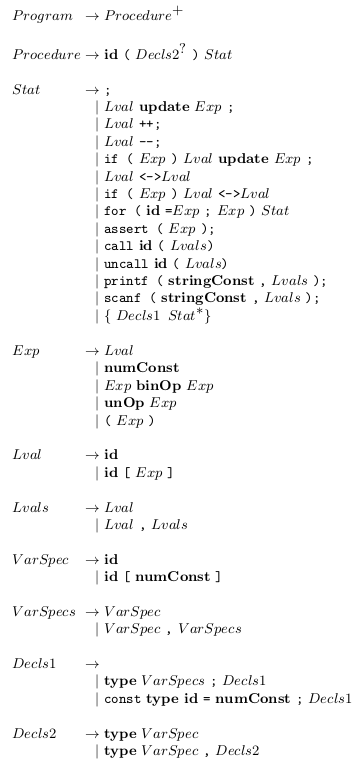
\includegraphics[width=0.6\linewidth]{figures/syntax}
\caption{Syntax of Hermes.}
\label{Hermes-syntax}
\end{figure}
\subsection{Side-channels in Hermes}
One type of side-channel that can be problematic in cryptography is residual information left in memory after running the program. Such information might contain keys, partially or in their entirety, or pieces of the plaintext that was encrypted. This is problematic but is avoided in Hermes by having all variables returned to zero before executing the program. This zeroing of variables serves another purpose, apart from avoiding data-based side-channels, as it also helps with reversibility. Consider a program that finishes by subtracting something from a variable to zero it. When running in reverse, the inverse of that operation would be to add that same value to the variable. 

%%%%%%%%%%%%%%%%%%%%% Check lige med michael om det er relativt nyt at angribe ved at kigge på timing. 
Another type of side-channel attack is timing-based side-channel attacks. Several precautions have been taken with Hermes to avoid such attacks, including:
\begin{itemize}
\item Not including time-sensitive control structures. This means that Hermes does not support \texttt{while}-loops, and that \texttt{for}-loops are restricted to iterating over a loop-local variable, which may only be updated with unconditional constant updates. 
\item Conditional updates are always evaluated. That is to say, that even if a condition is not true, the right-hand side of the update is still evaluated, to avoid value-dependent timings.
\item Logical operators like \texttt{\&\&}, \texttt{||} and \texttt{!} are not included in Hermes, only the binary equivalents.
\end{itemize}
There are more restrictions that the programmer needs to abide by when coding programs in Hermes. For a more comprehensive insight into the restrictions of Hermes, refer to \cite{PSI19}.

\subsection{Values in Hermes}
In Hermes there are three basic values to work with:
\begin{itemize}
\item Constants: These are initiated with a value and cannot be modified, which also means that they need not be zeroed before execution.
\item Variables: These may be integers, signed or unsigned, of either 8, 16, 32, or 64 bits. Variables must be zeroed before execution. 
\item Arrays: Elements must be of the same type as variables, and the size of arrays must be specified at declaration. Arrays, like variables, must be zeroed before exiting their scope. 
\end{itemize}
When working with arrays or variables, the values are never overwritten in fashions akin to:
\begin{verbatim}
u8 x = 3;
x = 4;
\end{verbatim}
Overwriting values like that is not reversible, so rather than overwriting, values are updated or swapped:
\begin{verbatim}
u8 x, y; // Values are initially zero.
x += 3;  // Assigning 3 to x by addition. 
y += 4;  // Assigning 4 to y by addition.
x <-> y; // Swapping the values in x and y. 
x -= 4;  // Reverting x to zero by subtraction. 
y -= 3;  // Reverting y to zero by subtraction.
\end{verbatim}
Here making sure to return the variables to zero before executing. 

%%%%%%%%%%%%%%%%%%%%%%%%%%%%%%%%%%%%%%%%%%%%%%%%%%%%%%%%%%%%%%%%%%%%%%%%%%%%%%%%%%%%%%%%%%%%%%%%%%%
%%%%%%%%%%%%%%%% Her er jeg nået til %%%%%%%%%%%%%%%%%%%%%%%%%%%%%%%%%%%%%%%%%%%%%%%%%%%%%%%%%%%%%%
%%%%%%%%%%%%%%%%%%%%%%%%%%%%%%%%%%%%%%%%%%%%%%%%%%%%%%%%%%%%%%%%%%%%%%%%%%%%%%%%%%%%%%%%%%%%%%%%%%%
%%%%%%%%%%%%%% Alt herunder er lidt bare gentagelser, så jeg har bare fjernet det. Vi mangler ikke ligefrem materiale. 

%Hermes is a reversible programming language specifically designed for encryption. Built with an offset in the reversible
%language Janus, Hermes has a C-like syntax.

% Should this be mentioned? I'm guessing it is mentioned elsewhere.
%The reversible manner implemented in Hermes makes it an adequate candidate to do so, due to the ability of decryption which be performed by running the encryption backwards.

% The reversible manner (get more in-depth)
%The original value of a variable is never overwritten. Alternatively, the value is either swapped to another temporary variable or updated reversibly.


%Importantance of talking about the semantic of Hermes this way?
%Values used in Hermes are either variables or one-dimensional arrays with elements representing signed and unsigned 32 or 64-bit two’s complement numbers

\subsection{Compiling Hermes}
\label{HC}
The original version of Hermes has had a compiler build for it. The compiler is built with Moscow ML\footnote{http://www.itu.dk/~sestoft/mosml.html}, so an installation of this is needed to build the compiler.

The source code for the compiler is included in the \texttt{src.zip} folder, along with a \texttt{Makefile} for building the compiler.

Provided a machine with Moscow ML installed, simply run the \texttt{Makefile} in the \texttt{Compiler} directory (not to confuse with the \texttt{Makefile} to compile the solution):
\begin{lstlisting}[language=C]
  $ make
\end{lstlisting}%$
This should create a \texttt{bin} folder, containing the compiler. 

Credit for the compiler goes to Malte Sølveste Velin and Sebastian Posselt \cite{Compiler}.
\subsection{Cryptography in a reversible manner}
\label{reverseCrypt}
% Nothing new here. Present some previous work on Hermes, and explain why cryptography has a particularly neat nature when it comes to reversibility. Asymmetric cryptography to come later.
Cryptography is, by nature, a reversible process. Text is obscured by encryption and then revealed again by decryption. Symmetric encryption embodies the very essence of reversibility, as decryption is exactly the inverse of encryption (hence symmetric). Extensive work has been done on symmetric encryption in Hermes. As an example, here is included the Tiny Encryption Algorithm (TEA)\cite{TEA} implementation in Hermes, presented in \cite{PSI19}, as well as the \texttt{C}-code from the Wikipedia page for TEA\cite{TEA}:
\begin{figure}[!h]\small
\begin{verbatim}
encrypt (u32 v[2], u32 k[4])
{
  u32 v0, v1, sum, k0, k1, k2, k3;
  const u32 delta = 0x9E3779B9;                   /* a key schedule constant */
  v0 <-> v[0]; v1 <-> v[1];                       /* set up */
  k0 += k[0]; k1 += k[1]; k2 += k[2]; k3 += k[3]; /* cache key */
  for (i=0; 32) {                                 /* basic cycle start */
    sum += delta;
    v0 += ((v1<<4) + k0) ^ (v1 + sum) ^ ((v1>>5) + k1);
    v1 += ((v0<<4) + k2) ^ (v0 + sum) ^ ((v0>>5) + k3);
    i++;
  }                                               /* end cycle */
  k0 -= k[0]; k1 -= k[1]; k2 -= k[2]; k3 -= k[3]; /* clear locals */
  sum -= delta << 5;                     /* alternatively, sum -= 0xC6EF3720 */
  v[0] <-> v0; v[1] <-> v1;                       /* return coded values */
}
\end{verbatim} 
\caption{Example of TEA implemented reversible in Hermes \cite{PSI19}.}
\end{figure}\\
\begin{figure}[!h]\small
\begin{verbatim}
void encrypt (uint32_t v[2], uint32_t k[4]) {
   uint32_t v0=v[0], v1=v[1], sum=0, i;          /* set up */
   uint32_t delta=0x9E3779B9;                    /* a key schedule constant */
   uint32_t k0=k[0], k1=k[1], k2=k[2], k3=k[3];  /* cache key */
   for (i=0; i<32; i++) {                        /* basic cycle start */
      sum += delta;
      v0 += ((v1<<4) + k0) ^ (v1 + sum) ^ ((v1>>5) + k1);
      v1 += ((v0<<4) + k2) ^ (v0 + sum) ^ ((v0>>5) + k3);
   }                                             /* end cycle */
   v[0]=v0; v[1]=v1;
}

void decrypt (uint32_t v[2], uint32_t k[4]) {
   uint32_t v0=v[0], v1=v[1], sum=0xC6EF3720, i; /* set up; sum is 32*delta */
   uint32_t delta=0x9E3779B9;                    /* a key schedule constant */
   uint32_t k0=k[0], k1=k[1], k2=k[2], k3=k[3];  /* cache key */
   for (i=0; i<32; i++) {                        /* basic cycle start */
      v1 -= ((v0<<4) + k2) ^ (v0 + sum) ^ ((v0>>5) + k3);
      v0 -= ((v1<<4) + k0) ^ (v1 + sum) ^ ((v1>>5) + k1);
      sum -= delta;
   }                                             /* end cycle */
   v[0]=v0; v[1]=v1;
}
\end{verbatim} 
\caption{Example of TEA implemented in C \cite{PSI19}.}
\end{figure}
\\
As seen in the example, when implementing symmetric encryption algorithms in a reversible language, as opposed to a regular irreversible language, only one method is needed in place of two (one for encryption and one for decryption).

This neat property is only applicable to symmetric encryption. When implementing asymmetric cryptography, there will still be a need for two functions, as encryption and decryption are not simply each other's inverses.
